\documentclass{article}
\usepackage[draft]{SRM2}
\usepackage{graphicx}
\usepackage{url}

\title{The AviaNZ Birdsong Analysis Software (v 2.0)}
\author{The AviaNZ Team \\(\url{stephen.marsland@vuw.ac.nz})}
\date{October 2019}

%\usepackage[usenames, dvipsnames]{color}

%Revise with track changes
%\usepackage[markup=default]{changes}
%\usepackage[final]{changes}
\usepackage{soulutf8}
\usepackage{todonotes}

\begin{document}
\maketitle

This is the user manual for version 2.0 of the AviaNZ program. The biggest change in this version is the way that species recognisers are trained and stored. There are a few other improvements, but the recognisers are the biggest change.
As well as this manual, there are  some short `How to' guides \todo{Maybe?} and videos available at \url{http://www.avianz.net}.
 
We really want feedback on AviaNZ, particularly what works and what doesn't, how you would like to see it improved, and what other functionality it needs. We are more than happy to talk about our plans as well. 

\tableofcontents

%If you haven't done any birdsong processing before, make sure that you read Section~\ref{labelling}, which works through an example. 

\section{Getting Started}

%{\em In contrast to previous versions, this version of AviaNZ does not require you to run it as administrator in Windows. It places some files in the home directory of your computer; in \url{C:/Users/username/AppData/Roaming/AviaNZ} for Windows and \url{~/.avianz} for Mac and Linux.}

AviaNZ has three main modes of interaction, which are presented as options on the start-up screen:

\begin{figure}[h!]
\centering
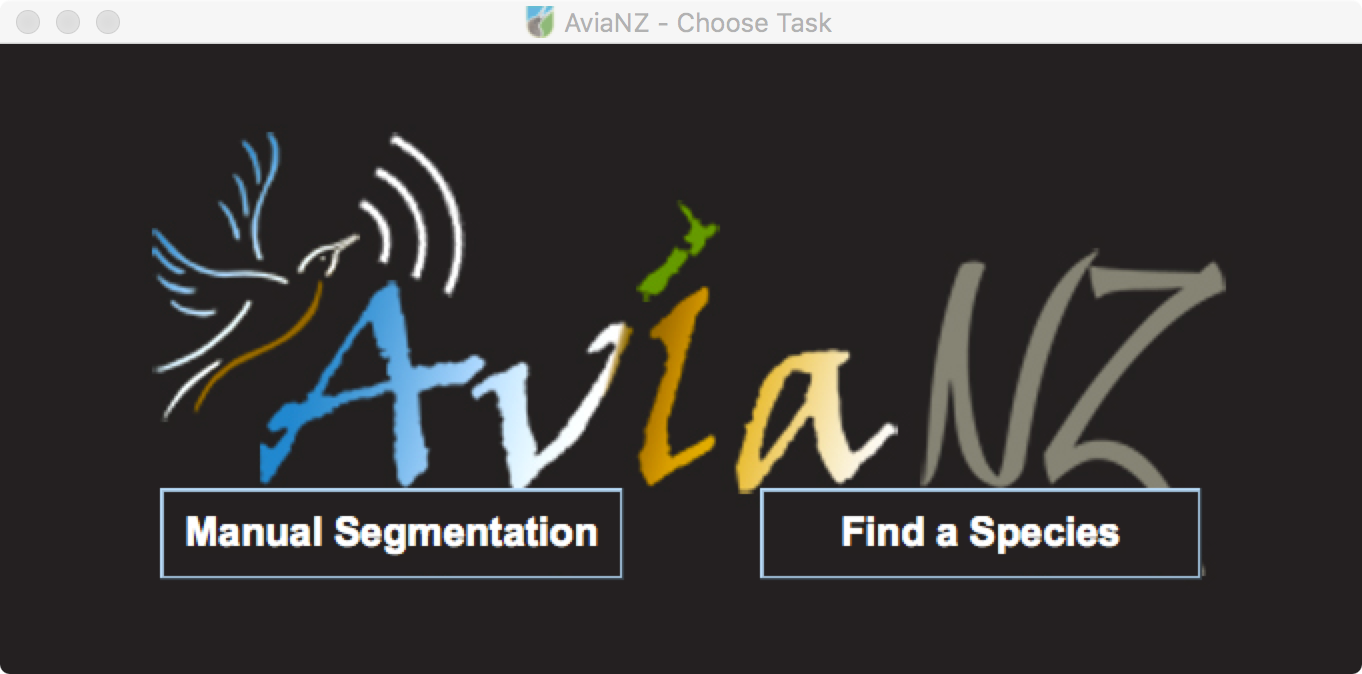
\includegraphics[width=.3\textwidth]{Figs/splashscreen}
%\caption{\added{Starting window of the program.}}
\label{welcome}
\end{figure}

The first option (`Manual Processing') is described more in Section~\ref{sec:manual}. It enables you to look at, listen to, and manually annotate individual audio files, as well as to train your own recognisers. The second option (`Batch Processing') takes whole directories (and subdirectories) of audio files and automatically segments the bird calls of selected species you have recognisers for; see Section~\ref{sec:auto}. You can view the output of the automatic segmentation using the the third option (`Review Batch Results', see Section~\ref{sec:review}), but if you want more context on them you could also use the first (`Manual Processing') option. 
The software also produces an Excel file showing the results; these are described in more detail in Section~\ref{sec:outputs}. 

\section{Manual Processing}
\label{sec:manual}

If you select `Manual Processing', you will see a dialog box asking you to select a file to view. Use this in the normal way to select a sound file from a directory. The program will ask you to give names for the operator and reviewer. These are useful to keep track of who has looked at different files. Following that, you should see a screen like the one below (Figure~\ref{main}). This is the main program for manually labelling birdcalls, training recognisers, or testing things. It can also be used for reviewing the processing of automatic processes; checking for misclassifications is usually easier in `Review Batch Results', but the manual processing mode also allows you to see if there are any calls that the recogniser missed. 

The program automatically loads the first 5 minutes of a file (if it is in wav format; mp3 files lose a lot of information and should not be used, other formats should be converted to wav before use). AviaNZ assumes that sound files are recording in mono (single microphone) sound. If there are other channels, it only loads the first one.

\begin{figure}[h!]
\centering
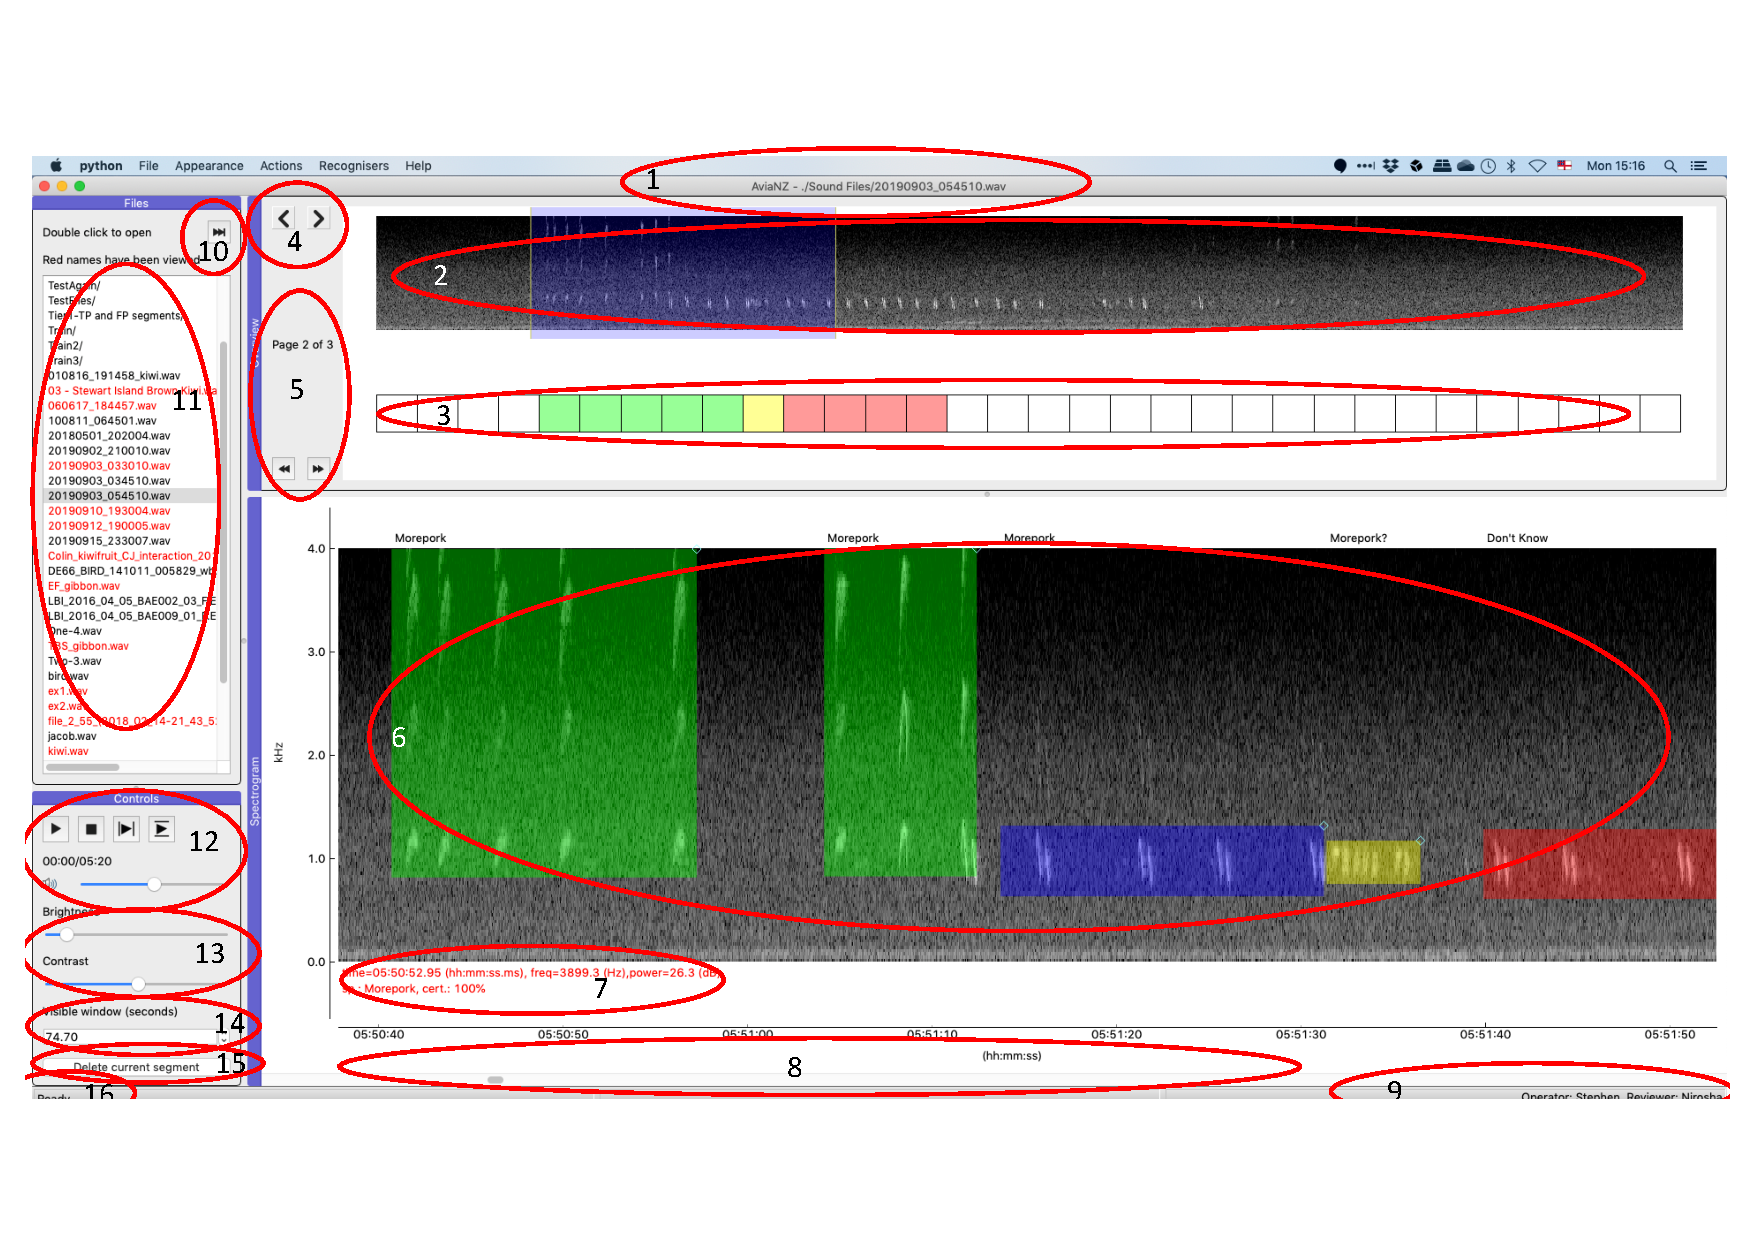
\includegraphics[width=.8\textwidth]{Figs/AviaNZInterface.pdf}
\caption{The interface for manual processing and analysis.}
\label{main}
\end{figure}

There are five separate areas of the screen within the `Manual Processing' part of AviaNZ. Each has its name in a blue bar. They are:
	\begin{description}
	\item[Overview] This shows you a picture of a 5 minute segment of the file (labelled 2 in the figure). The part you are looking at in the main plots is shown in blue (it's actually the whole file in the example figure). Below it there is a coloured bar (in yellow and labelled 3 in the figure). There are left and right arrow buttons (labelled 4) and double arrow buttons (labelled 5) on the left of this area. The single arrow buttons move the view in the main area along, while the double arrow buttons move to the previous 5 minutes or to the next 5 minutes of the file (if they exist). 
	\item [Files (11)] This is a list of files in your current directory. You can double-click on one to select it and open it. Files in red have been annotated, files in black have not. The double arrow button on the top right of this area (labelled 10) moves on to the next file.
	\item[Spectrogram plot (6)] This is the main representation of the sound file. It is possible to display information about where the mouse is pointing on the spectrogram (time, frequency, energy value; (7 in the figure)) by choosing `Show pointer details in spectrogram' from the Appearance menu, and to switch it off the same way. There is also a scroll bar to move through the file (8). 
	\item[Controls] These play the sound file, and modify the appearance of the plots (12--17 in the figure), see Section~ref{sec:controls}.
	\end{description}

There are two other parts to the interface:
	\begin{description}
	\item[Menu] The menu at the top of the screen. The name of the current file is shown in the title of the window (1).
	\item[Bar at the bottom] At the very bottom of the screen there is an area (18) that gives any status updates from the program, and on the right, information about the currently selected Reviewer and Operator (9).
	\end{description}

You can drag the five screen areas around and reorder them if you wish, by dragging the blue bar on the top or left of them. You can also make them into their own windows by double-clicking on the blue bar. If you decide that you made a mistake doing that, then there is an option in the Actions menu to `Put docks back' that returns them to the original configuration.

To load a new file, either choose `Open sound file' in the File menu, or just double click one in the Files screen area (double clicking on a folder will open that folder), or click on the button labelled 10 to move to the next file. 

If you want to move to a new directory, either use the `..' option at the top of the list of files to navigate around your computer's file system, or use the  `Open sound file' in the File menu.

To restart the program, for example so that you can start doing some batch processing, choose `Restart Program' from the File menu. To quit completely, choose `Quit'. 

%\item The program will tell you if it is doing anything by putting text in the area labelled 18. \added{The selected operator is shown at the bottom of the window (10).}

\subsection{Spectrogram Plot}

The main spectrogram plot (6) shows a section of a sound file. The part you are looking at is highlighted in blue in the top (Overview: 2) picture. If you want to see the amplitude plot as well, select the `Show amplitude plot' option in the Appearance menu. Select the option again to hide the amplitude plot again. You can also hide the list of files (11) and the annotation overview (2--5) in the same way. AviaNZ will remember your choice in future uses.

The axes of the spectrogram are time on the horizontal axis and frequencies on the vertical axis. The times will be true times if this information is available (such as when using DOC recorders), or time from start of file otherwise. 

Sometimes spectrograms don't look good initially, for example because of high noise. You can modify the brightness and contrast of the spectrogram using the two sliders (15). You can also use a different colour scheme, and invert the colour map (swap black and white), by choosing the relevant options in the Appearance menu. 

\subsection{Zooming and Scrolling}

The part of the file you can see can be changed by:
	\begin{itemize}
	\item dragging the scroll bar below the spectrogram (8)
	\item clicking on the left or right arrows on the right of the Overview picture (4)
	\item dragging the blue highlight in the Overview picture itself (2). 
	\item clicking on any of the boxes in the bar below the Overview picture (3)
	\item pressing the left or right arrow keys
	\end{itemize}
The amount of the file that you can see (the visible width) can be changed by either: 
	\begin{itemize}
	\item dragging the ends of the blue highlight in (2)
	\item changing the `Visible window width (seconds)' in the Controls dock (16) by clicking on the up and down arrows, or typing in a new number.
	\end{itemize}

You can also view a restricted amount of the spectrogram by reducing the visible frequency band. To do this non-destructively, use the `Change spectrogram parameters' dialog in the Appearance menu, and change the Lowest and Highest Frequency options. There are other options in that dialog too. For more information about them, see Section~\ref{sec:spectrogram}.

\subsection{Moving Through Long Files}

If files are longer than 5 minutes, use the double arrows labelled (5) to move to the next or previous sections, or press shift + left or right arrow keys. Note that there is (by default) a 10 second overlap between the files. You can change the page size and the amount of page overlap by choosing the relevant options in the `Interface Settings' in the Interface menu, as will be described later. The times on the axis below the spectrogram show locations in the full file. Note that operations like denoising and segmentation (described in Section~\ref{sec:action}) apply to the visible 5 minute portion of the file, not the whole file. 

\subsection{Playing the Sounds \label{sec:play}}

You can play the sounds visible on the screen using the `Play' button at the top-left of the Controls section (labelled 12). The button turns into a `Pause' button while playing (or you can press the `Escape' key to pause playback). The light blue bar in the spectrogram plot (6)  shows where the playback is up to. When paused, you can drag this bar if you want to hear a particular part of the file. Move the mouse over it, and the bar will go red. Then click and drag (using the mouse button that does not make segments, by default the right button) to move it. The time below the play button shows the length of the file and the current position of the blue bar in minutes and seconds. You can change the volume of playback using the slider in (15). You can also play a segment of sound, assuming that a segment is selected. We will cover this below.

To stop playback and have the slider return to the start of the visible section, press the Stop button instead.

When a segment is selected (so that it is blue -- segments are covered next) you can use the two play buttons (labelled 13 in the picture) to play just that small segment. The difference is that the one on the left plays all the frequencies in the sound file, while the one on the right will play only the frequencies highlighted, so that you can isolate particular frequencies of a call. This is particularly helpful when there is high level of background noise in a particular frequency range, such as cicadas, or where there are overlapping calls in different frequency bands.

\subsection{Manual Labelling}

You select and edit a previously made segment by clicking on it with one of the mouse buttons,  and create one by using the other mouse button. The default is that segments are made with the left button and selected using the right button (pressing control on the keyboard when clicking on a Mac). You can select which mouse button performs which action using the `Mouse settings' of the `Interface settings' in the Appearance menu. 

If you select a segment that already exists by clicking on it then it will turn blue. Click on it again and the menu will reappear so that you can correct mistakes.

To choose the type of bird, click on the name. If the type isn't in the list, move to `Other'. If it isn't in the second list, at the bottom of that list is a selectable box (it probably says `Albatross'). Clicking on it provides the complete list of birds. If there is something missing from there, choose Other' from it, which is at the very end. It will ask you to enter a name, as Genus (Species); e.g., `Kiwi (Little Spotted)'. If there is only a single example of the genus, you can miss out the species, e.g., `Kakapo'. From then on this name will appear in the list. If you click anywhere on the screen except on a bird name in the menu then the menu will disappear and the bird type will be labelled as `Don't Know'. 

There are three options for how to create a segment. You select one of them in the `Mouse settings' of the `Interface settings' in the Appearance menu:
	\begin{itemize}
	\item {\em (default)} Drag a limited frequency band box (i.e., click and hold the mouse button and drag the mouse to the correct end point in both time and frequency)
	\item Start and stop a limited frequency band by clicking (i.e., click once at the correct time and frequency (in the spectrogram) for the start of a segment, and then again at the time and frequency for the end)
	\item Start and stop a full frequency band by clicking (i.e., click once at the correct time for the start of a segment, move the mouse to the end, click again, the box covers all frequencies)
	\end{itemize}

While the segment is being made, it is red. At the end it will turn blue, and a drop-down menu will then appear asking you to label the segment. 

By default the lists of bird names update dynamically, so that bird types you have chosen appear at the top of the list. If you don't like that, then you can disable it in the `Interface settings'. 

When creating a segment, you can give it the same label as the previous segment by pressing the shift key on the keyboard when you click to finish the segment. The program will then give the segment the same label as the previous box that you labelled, without showing you the list. This is very useful when there is one bird calling repeatedly.

You can also show that you are uncertain by pressing the control button when you click to segment (command button on a Mac computer). The names of the birds will then have a question mark after them. 

By default, the software only allows one bird type to be specified for each segment. However, there may be times when you wish to label multiple species in one box (for example, for the dawn chorus). In that case, choose `Default to multiple species' in the `Interface settings'. Now, when you choose a bird from the list it will be ticked, and the menu will not close automatically, allowing you to make multiple selections. To unselect something, click on it again. When you make a new segment, `Don't Know' is selected by default. Choosing any other option deselects `Don't Know'. You can reselect it if you do want that label as well. 

If you find that the colours make it hard to see the data underneath the boxes you can make them transparent using the `Make dragged boxes transparent' option under `Annotation' in the `Interface settings'. You can also choose different colours if you have particular preferences.

You can denoise a single segment by selecting it, and then pressing the button with a paintbrush on in the `Controls' section (14). 

%\item The button with a small `i' on in the `Controls' section (14) changes the information that is shown about each segment; rather than the species label, the syllable name from the recogniser is given. The drop-down list then changes to enable you to correct this instead if there are any options to do so. 

The segments that are drawn on the screen have different colours. These colours are changeable in the `Interface settings', but by default are:
	\begin{description} 
	\item[Blue] This segment is currently selected. You can play it by pressing the buttons in 12, or give it a new label, or delete it using 16. 
	\item[Green] This segment has been labelled with a bird name.
	\item[Yellow] This segment has been labelled with a bird name with a question mark.
	\item[Red] This segment has been labelled as `Don't Know'.
	\end{description}

These colours match the rectangles underneath the overview (3). For each 10 second segment of the file, these boxes are:
	\begin{description} 
 	\item[White] if there are no segments, 
	\item[Red] if there are `Don't know' segments, 
	\item[Yellow] if there are question-marked segments, or 
	\item[Green] if all the segments in that section are labelled with definite species. 
	\end{description}
	
You can click on the rectangles in (3), and they will update the main spectrogram plot to show that section of the file. This is a good way to move through the file quickly.

A segment that has been selected can be moved by dragging it, or resized by dragging the handle on the top right corner of the box. (All these interactions use the non-drawing mouse button.)

Segments can be deleted by selecting them (so that they turn blue) and then clicking on the `Delete Current Segment' in the Controls (16). You can also just press the delete or backspace key on the keyboard. 

To delete all of the segments, use the `Delete all segments' option in the Actions menu. 

Segments are saved automatically, so that you can't lose your work.


\subsection{Menu Options}	

\subsubsection{{\em File Menu}}

\begin{description}
\item[Open sound file] Produces a file dialog so that you can choose a new sound file to open.
\item[Set operator/reviewer] Enables you to change the operator or reviewer for this file only. 
\end{description}

\subsubsection{{\em Appearance Menu}}

\begin{description}
\item [Changing appearance] The first four options in the menu hide or reveal the amplitude plot (6), list of files (12), annotation overview (3), and information about where the mouse is pointing in the spectrogram (8). 
\item [Choose colour map] This enables the user to select a colour map they prefer to the standard grey one. 
\item [Invert colour map] By default, areas of high energy (frequencies where there is a call or other sound) are shown as the lightest colour, and low energy as dark. This can be swapped over with this option. Note that you will need to change the brightness and contrast then. 
%\item [Make frequency axis tight] After bandpass filtering, this updates the spectrogram plot to stop showing the empty bands.
\item [Change spectrogram parameters] A set of options to modify the spectrogram. Enables changes of the windowing function, width and increment of the FFT, and the option to not subtract off the mean. See Section~\ref{sec:spectrogram} for more details. %The `Multitapering' option can make very noisy spectrograms look better, but it takes a lot of computer time. 
The two sliders at the bottom of the dialog enable the user to non-destructively show a limited frequency band in the spectrogram. The axis in the plot shows the range that is visible. 
\item [Mark in spectrogram] There are some features that call help you spot bird calls or recognise them. We currently offer two options here: the fundamental frequency, and high spectral derivatives. See Section~\ref{sec:spectrogram} for more details.
\item [Make read only] When reviewing a segmentation it is possible to click on the plots by mistake, adding further segments. This option avoids this problem. It can be turned off by selecting it again. When read only mode is on, the message section in (18) says so. 
\item [Interface settings] This option produces a dialog that enables the user to customise several things about AviaNZ. In particular:
\begin{description}
\item[Mouse settings] Swap which mouse button selects segments and which creates them, and change the method of creating segments (clicking or dragging).
\item[Paging] The page is the length of spectrogram loaded into AviaNZ at one time. By default it is 300 seconds (5 minutes). Note that longer times will require more memory and processing time. The amount of overlap between the pages can also be specified. The aim of the overlap is to make sure that calls aren't missed, and that segments are labelled accurately, at the page limits. 
\item[Annotation] The first option in this section changes the length of the boxes labelled (3) in the figure. The next enable you to change the colours of the segments. They can also be made transparent (so that only the outline of the box is shown) if you find it hard to see what is in a segment. Finally, AviaNZ has a check-ignore protocol for people who only annotate subsets of recordings. This puts a mark on the spectrogram in places where the user should be annotating the spectrogram. 
\item[Bird list] There are two bird lists in AviaNZ: the short list of common birds, and a longer list of all possibilities. You can change these files for others (for example, to include non-New Zealand species). See Section~\ref{sec:birdlists} for more information. You can also change the default behaviours of dynamically updating the list of common birds, and enable multiple species to be selected for a single segment. This can be useful for labelling things like the dawn chorus, but these segments will not provide good training data for new recognisers. 
\item[Human classify] By default, AviaNZ saves corrections that are made using the review options (see Section~\ref{sec:review}). 
\item[Output parameters] By default, AviaNZ save the segments you have made every 60 seconds. This can be changed, for example if you want to do it more often for safety.
\item[User] Enables you to set the operator and reviewer; this facility can also be found in the File menu. You can also change whether or not the AviaNZ window starts at full screen size, and whether or not the noise data must be completed for all files. 
\end{description}
\end{description}

\subsubsection{{\em Actions Menu}}
\label{sec:action}

These options will mostly provide dialog boxes that ask you to make choices. 

\begin{description}
\item [Delete all segments] Does what it says. 
\item [Denoise] Runs some programs that try to get rid of the noise in the sound file so that the birdcalls are easier to see. See Section~\ref{sec:denoising} for more information.
\item [Add metadata about noise] Allows the user to specify if the sound file is particularly corrupted by noise, and also to identify the type(s) if known. This can be an optional datafield, or made compulsory for each file by choosing the appropriate option in the `Interface settings'.
\item [Segment] You can ask the computer to segment the calls automatically. We currently provide 3 options. The first (`Wavelets') applies a pre-trained recogniser for a particular species, in the same way that the Batch Processing mode (Section~\ref{sec:auto}) does, but just to the current page. The other two (`FIR' and `Median Clipping'; see Section~\ref{sec:segmentation}) will create a segment for any significant noise in the file. 
%\item [Find Matches] If you select a segment (so that its box is green) and then press this button the program will look for others that are similar. It does not currently deal well with nosie. 
%\item [Filter Spectrogram] This tries to clean the spectrogram for easier viewing.
\item [Human Review] These two options provide two different ways to view the segments and their labels on the current page for easier checking. For more, see Section~\ref{sec:batchreview}.
\item [Export segments to Excel] This enables the user to save a summary of the annotation of the currently opened file into an Excel workbook (in the same location as the current sound file), as is described in Section~\ref{sec:outputs}. 
\item [Save as image] Saves the spectrogram currently visible on the screen as an image, including any segments marked. 
\item [Save selected sound] Saves a selected segment as a short sound file.
\item [Put docks back] Returns the various screen components to their original layout if they have been moved around. 
\end{description}

\subsubsection{{\em Recognisers Menu}}

\begin{description}
\item [Train a species recogniser] A significant new feature of this version of AviaNZ is that you can now train your own species recognisers. The process is relatively simple, and is described in Section~\ref{sec:trainfilter}.
\item [Test a species recogniser] Enables you to test a recogniser by choosing a folder to run it on. See Section~\ref{sec:testfilter}.
\item[Manage recognisers] Lets you rename, export, or import new recogniser for different species. See Section~\ref{sec:filters} for more details.
\end{description}

\subsubsection{{\em Help Menu}}

\begin{description}
\item [Help] Gives access to this manual online.
\item [Cheat sheet] Links to our webpage to see examples of New Zealand bird spectrograms and calls, mostly taken from New Zealand Birds Online.
\end{description}

\section{Batch Processing}
\label{sec:auto}

Batch processing is for use when you have large numbers of recordings that need to be processed, for example when you collect recorders from the field. Download all of the data from the SD cards onto your computer, and then start AviaNZ. 

Select `Batch Processing' from the starting window. You will see a screen like the one shown in Figure~\ref{batch}. Navigate to a folder containing recordings to process. If this folder contains subfolders, the program will work through all of the folders inside the original one. It ignores any files that already have annotations. \todo{Is this true?} There are two outputs from batch processing: the data files that AviaNZ uses to label segments, and Excel files annotating the presence or absence of different species (see Section~\ref{sec:outputs}).

\begin{figure}[h!]
\centering
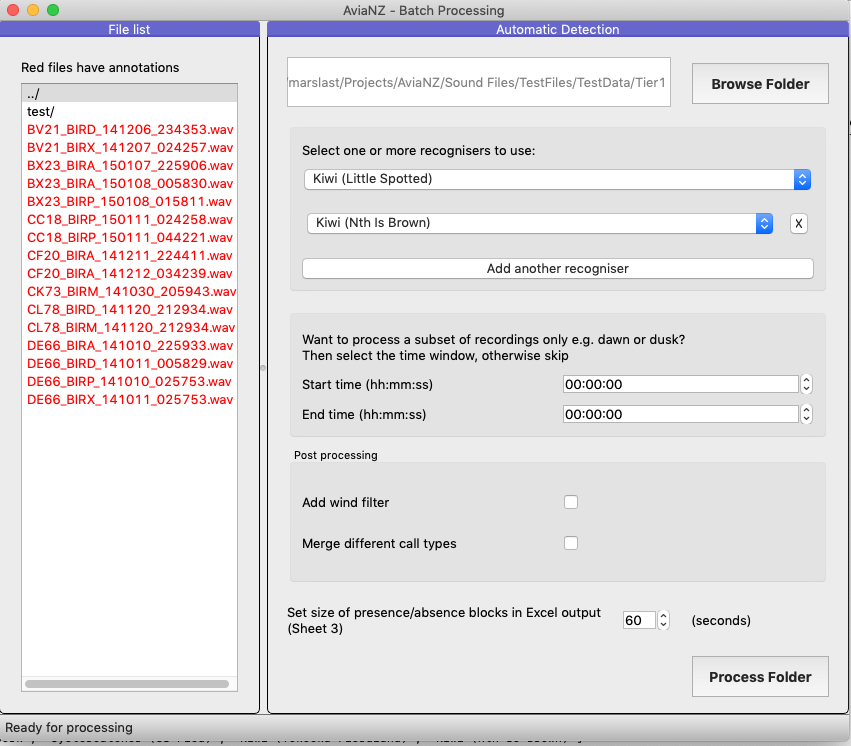
\includegraphics[width=.5\textwidth]{Figs/Batch1}
\caption{The interface for batch processing.}
\label{batch}
\end{figure}

You can choose one or more species-specific recognisers from the drop-down list to apply to the sound files in order to automatically label them. Alternatively, you can select `Any sounds'; in this case AviaNZ will show any sounds in the files, and label them as `Don't Know'. \todo{Correct label?}

For recordings from DOC recorders you can also choose to limit the times of the recordings. 

AviaNZ also produces an Excel spreadsheet, as is described in Section~\ref{sec:outputs}. One sheet of this spreadsheet shows Presence/Absence in time blocks. You can set the length of this time block here.
Note that the `Any sounds' option will delete the Excel files for individual species to ensure that everything is consistent. The information is then held in the one spreadsheet.  
%\item Something about post-processing options?

Press the `Process Folder' button to start the program. Note that this is a very computationally intensive process, and will take a long time (hours) if there are lots of files to process, and make your computer hard to use for anything else. It is generally best to leave it overnight.

If you stop the processing partway through, AviaNZ will try and restart from the place it got up to last time if you restart it.

Once it has finished, the window will give you the option to see the AviaNZ start screen again so that you can review the outputs. You can either do this in the `Manual Processing' interface, or use the `Review Batch Results' option, which is described next. 

\section{Review Batch Results}\label{sec:review}

A similar menu to the `Batch Processing' option will prompt you to select a folder with previously processed files. There are two forms of review in AviaNZ. 
If you choose `All species' then you will see a screen like Figure~\ref{check1}, while if you select a particular species, you will see a screen like Figure~\ref{check2}. You can also see these two types of review from the `Manual Processing' interface by selecting `Human review' and then either `All segments' or `Choose species'. 

The first option shows the labelled segments one-by-one using the interface shown in Figure~\ref{check1}. 
The green bars on the spectrogram show the start and end of the call, the spectrogram includes a couple of seconds of context sound too. Make the window larger if the spectrogram is too large for the window, or use the `+' and `-' buttons. You can play the sound with the play button. You can also change the spectrogram brightness to make it easier to review. If the label is correct, click on the green tick, which will make the next image load. If not, select the correct label before clicking the tick button. If you have allowed multiple species selection you can pick several options. To delete a segment, click on the red dustbin button. To move back to the previous one, click the back arrow; note that this will not save your current changes. 

	\begin{figure}
	\centering
	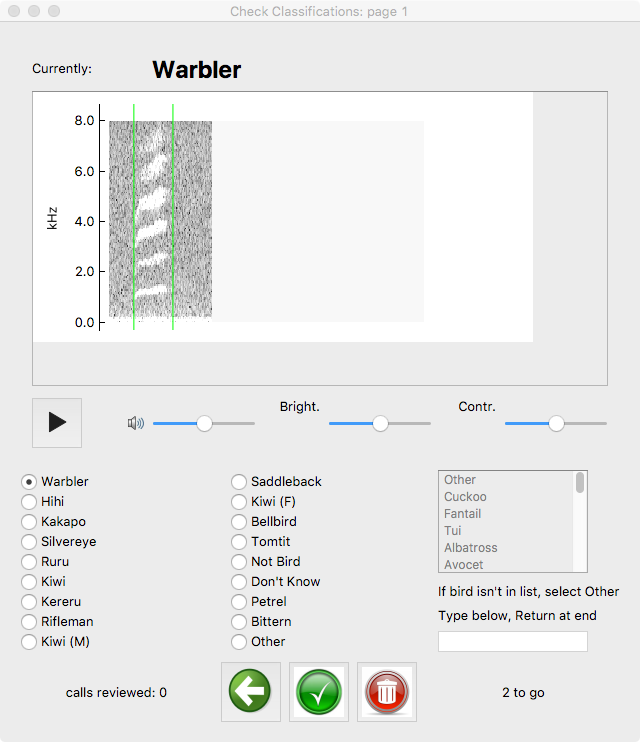
\includegraphics[width=.6\textwidth]{Figs/review1}
	\caption{Example of outputs for Human Review [All segments].}
	\label{check1}
	\end{figure}
	
The second option (Figure~\ref{check2}) requires you to choose a species from those found in the current file. It will then show a set of spectrograms from the file that have all been labelled as that species. Make the window larger to see more of them. For each segment that is wrongly labelled, click on its picture (it will be marked with a cross). If you click on it again, the cross will become a question mark to show that you are unsure, and if you click again, it will return to having no mark. Segments marked with a cross will be deleted. If you click again, it will be marked with a question mark, and if you click again then it will cycle back to being accepted. You can change the brightness and contrast here as well, and also play the sounds by hovering on the image, and then clicking on the play button when it appears. The `Toggle all' button cycles all of the spectrograms through the cross-question mark-OK stage, so that you don't have to click on every button if there are a lot of errors. Click on `Next' to move on to the next screen. 

	\begin{figure}
	\centering
	\includegraphics[width=.4\textwidth]{Figs/review2_2}
	\caption{Example of the window for Human Review [Choose species].}
	\label{check2}
	\end{figure}
	\end{description}

\section{Outputs}
\label{sec:outputs}

The AviaNZ program aims to provide detailed and easy-to-review outputs. An Excel file (with the name `DetectionSummary' followed by species selected) will be generated with three sheets of outputs in the same directory as the files. If this file already exists, the new results will be appended to the end of each sheet. 

The three sheets of the Excel workbook are:
\begin{enumerate}
\item start and end times of each birdcall detected
\item presence/absence of the target species (or set of species) in each recording
\item  presence/absence of the target species (or set of species) in each time interval that the user specifies (by default 60 seconds)
\end{enumerate}

In addition to the Excel file, for each sound file AviaNZ generates an annotation file of the automated detections that  the user can open and review in either the main interface or using the `Review Batch Results' option. 

\section{Training a species recogniser}\label{sec:trainfilter}

\subsection{Overview}

One of the main features of AviaNZ is that you can train you own species recognisers, and swap them between people quickly and easily. At the moment these recognisers are fairly simple; they are intended to include {\em any} sound that might be a call from the species of interest. However, over time we will be working to improve them so that they are more accurate, while still being easy to train. 

There are three parts to training a filter:

\begin{enumerate}
\item Creating training labels
\item Running the training process
\item Testing the filter
\end{enumerate}

Once these have been completed, the filter will be saved, and can then be used in the recognition process, for example in `Batch Processing'. 

Before we start considering the process of training, it is useful to understand how to interpret the outputs that AviaNZ gives you. 

\subsection{Some important concepts}\label{sec:metrics}

The way that AviaNZ decides whether or not it has recognised a call correctly is by comparing it with human annotation. The training sounds files that you provide, together with their annotations, are used to recognise the characteristics of the calls of a particular species. Comparing the human and machine outputs, there are four possible outcomes for each second of the recording:

\begin{description}
\item[True Positive (TP)] AviaNZ and human agree that there was a call 
\item[True Negative (TN)] AviaNZ and human agree that there was not a call
\item[False Positive (FP)] AviaNZ says that there was a call, but the human did not
\item[False Negative (FN)] AviaNZ did not detect a call that the human found
\end{description}

The counts of how many seconds of the recordings correspond to each of these four quantities can be combined to produce a variety of measures of accuracy. Two of them are particularly important for us:

\begin{description}
\item[Specificity (True Negative Rate)] $= \frac{TN}{(TN + FP)}$ (number correctly labelled as negative / number labelled as negative)
\item[Recall (Sensitivity or True Positive Rate)] $= \frac{TP}{(TP + FN)}$ (number correctly labelled as positive / number correctly labelled) 
\item[False Positive Rate] $= 1 - \mathrm{Specificity} = \frac{FP}{(FP + TN)}$ (number incorrectly labelled as positive / number labelled as negative)
\item[Precision] $= \frac{TP}{(TP + FP)}$ (number correctly labelled as positive / number labelled as positive)
\end{description}

Ideally both recall and precision would be close to 100\%, but it is hard to do both at once. For this first part of the recognition process we aim to detect as many of the calls as possible (high recall), which can lead to lower precision. 

We also compare the True Positive Rate and False Positive Rates to assist in parameter setting, as we shall see shortly.

\subsection{Labelling}

The selection of sound files for training, and the careful labelling of the calls within those sound files, has the most potential for making a good recogniser. You should try to pick sound files that display all of the calls of that particular species. If the species shows geographical variation you should also pick them from across that range (or name the recogniser so that the geographical specialisation is clear).  Ideally you will need a few (5--30) examples of each type of call that the species makes. The sound files can have noise in them, although preferably not too much. It is helpful if you have both loud and quiet calls. Ideally you should avoid recordings where there are simultaneous calls from other species in the same frequency range. It is also a very good idea to have a set of different files for testing. The amount of testing data should be similar to the training data, and also include all the call types.

Once you have a few sound files, make new folders on your computer, for training and testing files, and copy the sound files into them. Then open each file in the `Manual Processing' interface of AviaNZ and manually label every call from that species with the species name. It is quite important to label every call from that species. Drag the box around the call reasonably accurately. For birds with calls, mark the whole call of one bird with a single box. Include any harmonics that are visible. If you have more than one bird of the species calling, mark them both, using separate boxes. If the calls overlap, the boxes can too. Do the same process for both the training and testing folders.

\subsection{The training process}

To begin training a recogniser, select `Train an automated recogniser' from the Recognisers menu. Then follow the instructions to select the folder, and the name of the species. There are a few places during the process where you can modify choices that AviaNZ has made. One is on the first page, where it says `Preferred sampling rate (Hz)'. If you don't know what these things mean, you can ignore them, but for experienced users, they are places where choices that AviaNZ has made might be improved upon. 

Once the initial choices have been made, AviaNZ will try to cluster your labelled training segments into groups of similar sounds, which it will show in an interface like the one in Figure~\ref{fig:clusters}. We will improve this clustering over time, but at the moment it does make errors. It can be helpful to give names to each cluster (such as the type of call, or sex of the caller) by clicking on the name and typing a new one. Also, correct any errors by clicking on the calls so that they get a tick on them and selecting the correct cluster from the drop-down box next to `Move Selected Segment/s to Cluster' and clicking `Apply'. You can play the calls by clicking on the top-left corner of them. 

AviaNZ will now work through each cluster, and train an individual recogniser for that kind of call. It will show you a variety of parameter settings; if you don't know what they are, just ignore them. The program will then search for good ways to represent those calls, which can take a while, and then show a plot of error rates for different parameter settings. This is known as an ROC curve, and it is a plot of the recall (True Positive Rate) against the False Positive Rate for different parameter settings; two examples are shown in Figure~\ref{fig:ROC}. The perfect recogniser would be in the top-left corner of the graph; points lower down miss examples of the bird calling, which calls further to the right provide a lot of false detections, i.e.., think the bird is calling when it is not. You need to choose the compromise between these two that you are prepared to accept: more work in reviewing to get rid of false positives, or accepting that the software has not detected every call. To make the choice, click near the point that you think is the best compromise on the curve. You don't have to click on it exactly, AviaNZ will show you which point is closest to where you clicked. You need to do this for each call type. 

In the Post-processing window, there is the potential to make another practical choice, which is whether or not to use the Fundamental Frequency calculation as part of the filter. For some calls, birds can produce a base note and then harmonics above that, and the fundamental frequency calculation tries to find the base note. Where this works it can be helpful, so if you compare the number of training segments where the software found a fundamental frequency with those where it didn't, you can see whether or not it makes sense to use it. You can also see the range of frequencies that were identified, so if they look wrong, don't use it. If you don't know, AviaNZ will try to work it out for itself. 

\subsection{Testing a recogniser}\label{sec:testfilter}

Following this, you should save the recogniser you have trained. It is then a very good idea to test it. If you have prepared testing data already, you can do this straight away, otherwise save the recogniser and then test at a later date by using `Test a recogniser' in the Recognisers menu. You should also test a recogniser that you receive from somebody else (for example, from our webpage) before relying on it.

Testing uses different sound files to the ones used for training. It runs the filter over the files, and compares the results to the human annotations using the same error metrics that were defined in Section~\ref{sec:metrics}. It gives a better indication of how well the recogniser will work in practice. If you look at the testing files after using this feature in the `Manual Processing' interface, you can see the annotations from both the human and machine in order to compare them. 

\subsection{Recogniser management}

You can rename, import, and export recognisers by using `Manage recognisers' in the Recognisers menu. If you have made recognisers for sounds that you think will be useful for other people, please email them to us. 

    \begin{figure}
    \centering
    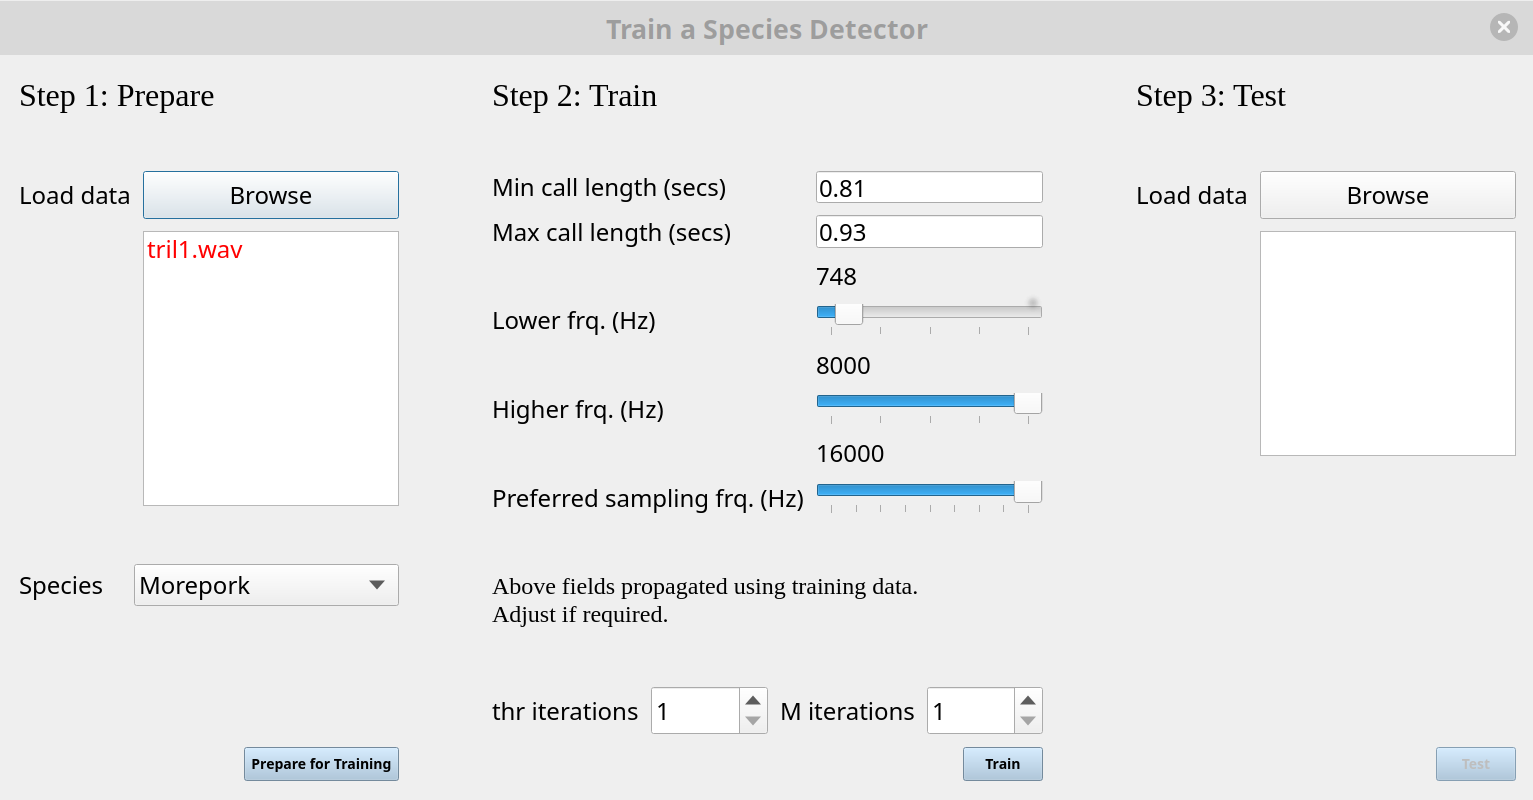
\includegraphics[width=.6\textwidth]{Figs/train}
    \caption{The dialog for training a species recogniser.}
    \label{fig:train}
    \end{figure}

    \begin{figure}
    \centering
    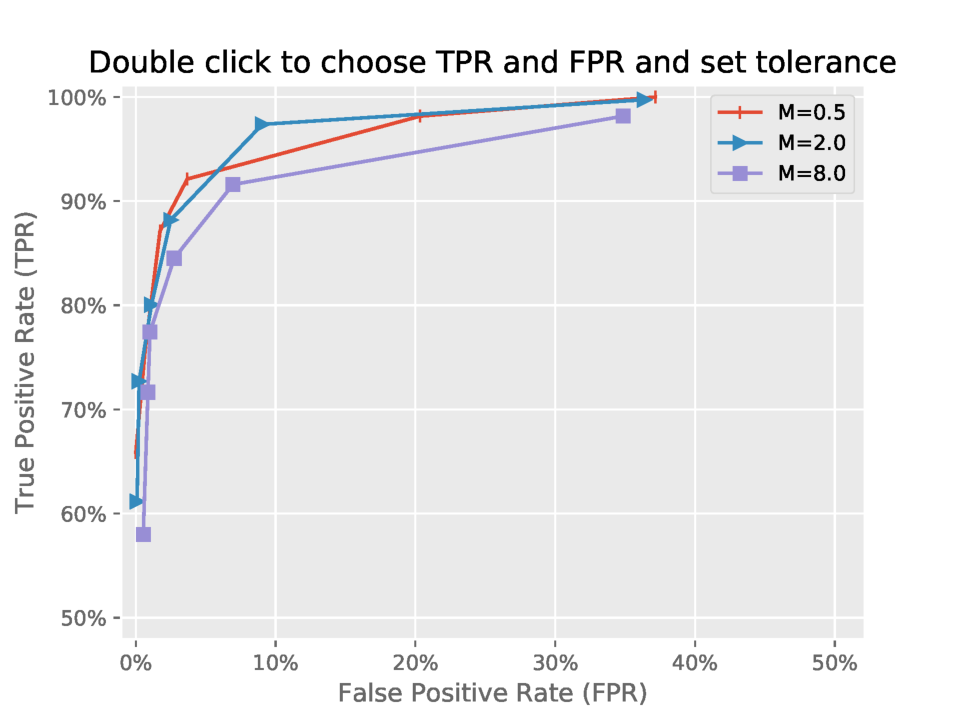
\includegraphics[width=.4\textwidth]{Figs/ROC_Curve_zoom}
    \caption{As part of the training process, AviaNZ will show a number of curves showing how different parameter values trade-off between false positives, and false negatives on the training data. A perfect classifier would be on the top-left of the plot, spotting every call and not labelling any other calls as your species. In practice, if you want to see every example of your species calling, the classifier will also make more mistakes where it labels other calls (or noises) as your species: false positives. This means that you will need to spend more time reviewing the outputs after using the recogniser. }
    \label{fig:selectfilter}
    \end{figure}
   
%
%\section{How Do I?}
%
%\subsection{Get started with manual labelling}
%
%\subsection{Deal with bird lists}\label{sec:birdlists}
%
%\section{Technical Details}
%
%\subsection{The Spectrogram}\label{sec:spectrogram}
%
%A spectrogram is actually a histogram plot of a short-time Fourier transform. A short segment of a sound file is multiplied (convolved) with a window function that makes it go to 0 at either end. The Fourier transform is then applied, the modulus  of the complex number taken and the value turned into decibels ($10 \times \log_10$). The amount of energy in each frequency band is plotted as a colour; in default AviaNZ the colour is black where there is no energy, and white at the highest energy. This is plotted as a vertical line of the spectrogram. Then the next segment of sound is taken, and the process repeated. There are three user-controllable parameters in this: (i) the window function, (ii) the width of the window, and (iii) the amount that the window moves between steps, which controls the overlap between the windows. All three of these parameters can be controlled in AviaNZ. Instead of using a single window function, it is possible to use a set of them, and average the results of convolving the signal with them. This is known as multi-tapering. It leads to a better estimate of the signal, but at a higher cost of computation. It can also be selected as an option in AviaNZ.
%
%Spectral derivatives 
%
%\subsection{Denoising}\label{sec:denoising}
%
%\subsection{Automatic Segmentation}\label{sec:segmentation}
%
%\subsection{Training}\label{sec:training}

\end{document}
